% =====================================================================
%  Data Engineering (34623) - Semester Project
%  Checkpoint 1: Dataset & Idea Validation - Written Status Update
%  Universidad San Jorge - Lecturer: Luis Palazón Simón
%  Compile with: latexmk -pdf checkpoint1_status_update.tex
% =====================================================================
\documentclass[11pt,a4paper]{article}

% ---------- Packages ----------
\usepackage[utf8]{inputenc}
\usepackage[T1]{fontenc}
\usepackage[english]{babel}
\usepackage{lmodern}
\usepackage[margin=2.3cm]{geometry}
\usepackage{booktabs}
\usepackage{tabularx}
\usepackage{enumitem}
\usepackage{xcolor}
\usepackage{tikz}
\usetikzlibrary{positioning,arrows.meta}
\usepackage{hyperref}
\hypersetup{colorlinks=true, linkcolor=blue!50!black, urlcolor=blue!50!black}

% ---------- Helper macros ----------
\newcolumntype{Y}{>{\raggedright\arraybackslash}X}
\setlist{nosep, leftmargin=*}

% ---------- Project metadata ----------
\newcommand{\projecttitle}{TETR.IO Player Progression Analytics}
\newcommand{\teamname}{Hueskers}
\newcommand{\submissiondate}{25/10/2026}
\newcommand{\repourl}{\url{https://github.com/inaTrip/tetrio-analytics}}

% =====================================================================
\begin{document}

% ---------- Title block ----------
\begin{center}
  {\Large\bfseries Data Engineering -- Semester Project}\\[4pt]
  {\large Checkpoint 1: Dataset \& Idea Validation}\\[8pt]
  {\large\itshape \projecttitle}\\[8pt]
  Team: \teamname \quad$\cdot$\quad Date: \submissiondate\\
  Repository: \repourl
\end{center}
\vspace{2mm}\hrule\vspace{4mm}

% =====================================================================
\section{Team and Roles}
\begin{tabularx}{\textwidth}{@{}lY@{}}
\toprule
\textbf{Member} & \textbf{Role (primary responsibility)} \\
\midrule
Eduardo Lázaro Esperón & Platform \& Cloud Lead \\
Hermes Benito Andrés   & Orchestration \& Quality Lead \\
Mariano Latre López    & Delivery \& Presentation Lead \\
All members (shared)   & Ingestion \& Storage \\
\bottomrule
\end{tabularx}

\medskip
\noindent Roles define internal ownership of tasks only; all members are
expected to understand and defend the complete solution.

% =====================================================================
\section{Project Idea}
\paragraph{Problem statement.}
TETR.IO's public API exposes the \emph{current} state of each player
(rating, rank, statistics) but no daily history, so it is not possible to
follow how a player progresses over time or which playstyle metrics are
associated with improvement.

\paragraph{Main question.}
\emph{How have competitive TETR.IO players progressed between 2023 and 2026,
and which playstyle metrics (APM, PPS, VS) distinguish the top rank tiers?}

\paragraph{Data product.}
A daily pipeline that snapshots the Tetra League leaderboard, integrates it
with a historical 2023 snapshot of the same players, and loads the result
into a dimensional data warehouse that feeds an insights dashboard.

% =====================================================================
\section{Selected Datasets}
\begin{table}[h]
\centering
\small
\begin{tabularx}{\textwidth}{@{}>{\raggedright\arraybackslash}p{2.2cm}YY>{\raggedright\arraybackslash}p{1.6cm}>{\raggedright\arraybackslash}p{1.4cm}>{\raggedright\arraybackslash}p{1.8cm}@{}}
\toprule
\textbf{Dataset} & \textbf{Content} & \textbf{Source / access} & \textbf{Update freq.} & \textbf{Format} & \textbf{Size} \\
\midrule
D1 -- TETR.IO API &
Tetra League leaderboard: rank, TR, Glicko, RD, APM, PPS, VS, games played/won, country &
\href{https://tetr.io/about/api/}{tetr.io/about/api}, Python \texttt{requests} &
Live (snapshot daily) &
JSON &
paginated (100 players/page) \\
D2 -- TETR.IO Player data &
Snapshot of all Tetra League players, September 2023 &
\href{https://www.kaggle.com/datasets/inferno2332/tl-data}{Kaggle}, \texttt{kaggle} Python API &
Static &
CSV &
45{,}197 rows, 16 columns, 6.3\,MB \\
\bottomrule
\end{tabularx}
\caption{Datasets selected for the project.}
\end{table}

\noindent\textbf{Licences and terms of use:}
\begin{itemize}
  \item \textbf{D1:} TETR.IO API usage rules: do not saturate the API
        (limit of about one request per second, with short bursts allowed),
        respect the cache times, identify the client with a
        \texttt{User-Agent} header, and use an \texttt{X-Session-ID} header
        for large series of related requests (never reused for unrelated
        requests).
  \item \textbf{D2:} Public Domain.
\end{itemize}

% =====================================================================
\section{Relatedness: How the Datasets Combine}
\begin{center}
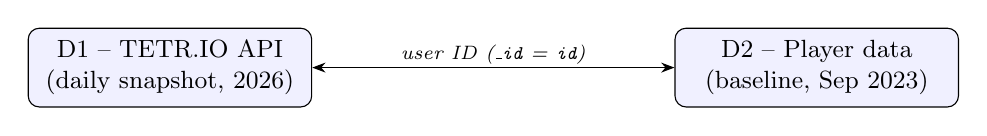
\begin{tikzpicture}[
  ds/.style={draw, rounded corners, fill=blue!6, minimum width=3.6cm,
             minimum height=1cm, align=center, font=\small},
  key/.style={font=\scriptsize\itshape, fill=white, inner sep=1pt},
  >=Stealth]
  \node[ds] (d1) {D1 -- TETR.IO API\\(daily snapshot, 2026)};
  \node[ds, right=4.6cm of d1] (d2) {D2 -- Player data\\(baseline, Sep 2023)};
  \draw[<->] (d1) -- node[key, above] {user ID (\texttt{\_id} = \texttt{id})} (d2);
\end{tikzpicture}
\end{center}

\noindent Both datasets come from the same platform. They share TETR.IO's
stable user identifier (\texttt{\_id} in the API, \texttt{id} in the CSV)
and the same statistics (TR, Glicko, RD, rank, best rank, APM, PPS, VS,
games played and won). The user ID is used as the join key instead of the
username, because usernames can change.

\medskip
\noindent\textbf{Validation performed.} Both datasets were profiled with
Python scripts stored in the repository (\texttt{notebooks/}):
\begin{itemize}
  \item D2 has no duplicate rows. Missing values appear only in
        \texttt{country} (1.0\%), \texttt{40l\_sprint} (11.6\%) and
        \texttt{blitz} (22.9\%), which correspond to players who never
        played those modes.
  \item A test fetch of the current top 500 players of the live leaderboard
        showed that 309 of them (62\%) already appear in the 2023 snapshot,
        so the join yields real progression data. Because the top of the
        leaderboard favours long-term players, the overlap for the full
        leaderboard is expected to be lower; it will be measured in the
        first full ingestion run.
\end{itemize}

\noindent\textbf{Third dataset.} A third dataset, Kaggle ``Tetr.io Top
Players Replays'' (MIT licence, which only requires keeping the copyright
notice), was evaluated and discarded: it contains no player
identifier, and all 76{,}692 games belong to the top rank tier (TR between
24{,}698 and 24{,}999), so it could not be linked to individual players or
used to compare rank tiers. Another third dataset is under evaluation
(candidates: per-player season history from the TETR.IO API, or
country-level World Bank indicators joined on country code).

% =====================================================================
\section{Relevance: Why These Datasets Fit the Requirements}
\begin{tabularx}{\textwidth}{@{}p{3.4cm}Y@{}}
\toprule
\textbf{Requirement} & \textbf{How the dataset choice supports it} \\
\midrule
Daily orchestration &
D1 changes continuously and keeps no daily history, so a daily snapshot is
the \emph{only} way to build the progression time series. \\
ETL \& warehouse &
Integration of a nested JSON source (D1) and a flat CSV source (D2) into a
star schema (Section~\ref{sec:model}). \\
Scalability ($\times10$ to $\times10^6$) &
Daily snapshots of all ranked players accumulate over time; volume growth
is estimated for each scale in the scalability analysis. \\
Insights &
Rating progression 2023--2026, rank vs.\ playstyle metrics, player churn. \\
Data consumers &
Players (progress tracking), tournament organisers (seeding),
community sites. \\
Privacy &
Usernames, country and activity patterns are personal data even if public.
API profiles also expose linked Twitch, Twitter and Discord accounts and a
biography; these are excluded at ingestion (data minimisation). \\
\bottomrule
\end{tabularx}

% =====================================================================
\section{Initial Data Model}\label{sec:model}
\begin{itemize}
  \item \textbf{Fact table:} \texttt{fact\_player\_snapshot}
        (TR, Glicko, RD, rank, APM, PPS, VS, games played and won;
        grain: player $\times$ snapshot date). The 2023 data is loaded as
        one historical snapshot; D1 adds one snapshot per day.
  \item \textbf{Dimensions:} \texttt{dim\_player} (slowly changing, type 2,
        to keep username and country changes), \texttt{dim\_date},
        \texttt{dim\_rank\_tier}.
\end{itemize}

% =====================================================================
\section{Risks and Open Questions}
\begin{itemize}
  \item \textbf{API limits:} the usage rules allow about one request per
        second, so a full leaderboard snapshot takes several minutes per
        day; requests are paced and the 10-minute cache is respected.
  \item \textbf{Rank system change:} the live API contains rank
        \texttt{x+}, which does not exist in the 2023 data, so rank tiers
        are not directly comparable across periods. Ranks are taken from
        the source rather than derived from TR thresholds.
  \item \textbf{Schema differences:} D1 contains fields not present in D2
        (\texttt{gxe}, \texttt{decaying}), which will be null for 2023.
  \item \textbf{Sentinel values:} the API uses \texttt{-1} for hidden
        counts (e.g.\ \texttt{gamesplayed}); these are converted to null in
        the transformation step.
  \item \textbf{Historical overlap:} part of D2 refers to players who are
        no longer active, which limits the joinable history.
\end{itemize}

% =====================================================================
\section*{AI Usage Disclosure}

In line with Section~8 of the project kickoff document, this section states
which parts of this deliverable were generated or assisted by AI.

\paragraph{Tool and model.}
Claude (Anthropic), model Claude Opus 5.5, used through the Claude desktop
application in October 2026.

\paragraph{1. Dataset search (assisted).}
\begin{itemize}
  \item \textbf{What was generated:} a list of candidate data sources for
        the chosen theme (Tetris), with a proposed role for each one in the
        warehouse, possible join keys, and risks to check. The AI ran web
        searches to find the sources.
  \item \textbf{Team contribution:} the theme was chosen by the team; the
        licences and API usage rules were read and summarised by the team.
\end{itemize}

\paragraph{2. Dataset validation scripts and interpretation (generated).}
\begin{itemize}
  \item \textbf{What was generated:} \texttt{notebooks/profile\_datasets.py},
        \texttt{notebooks/check\_rank\_join.py},
        \texttt{notebooks/test\_tetrio\_api.py} and
        \texttt{notebooks/test\_leaderboard.py}, plus the interpretation of
        their outputs (join key, overlap, data quality issues).
  \item \textbf{Prompts used:} ``Ok how do I know if the datasets are
        good?.
  \item \textbf{Team contribution:} the scripts were run by the team.
\end{itemize}

\end{document}